% XeLaTeX document
\documentclass[aspectratio=169, 11pt]{beamer} % для экранов 16:9 оставить

% \documentclass[11pt]{beamer} % для экранов 4:3 оставить

% Редактируем: конфигурация, личные настройки: имя, название предмета и пр. для титульной страницы и метаданных документа здесь
\newcommand{\university}{Московский государственный университет имени М.В. Ломоносова}
\newcommand{\faculty}{Факультет вычислительной математики и кибернетики}
\newcommand{\department}{Кафедра математических методов прогнозирования}
\newcommand{\city}{Москва}
\newcommand{\num}{ № 1}
\newcommand{\docname}{Построение поисковой системы для интернет магазина}
\newcommand{\tutorname}{д. ф.-м. н., профессор Дьяконов А.Г.}
\newcommand{\studentname}{Федоров И.С.}
\newcommand{\group}{417}

% Не редактируем: используемые пакеты
% настройка кодировки, шрифтов и русского языка
\usepackage{fontspec}
\usepackage{polyglossia}

% рабочие ссылки в документе
\usepackage{hyperref}

% графика
\usepackage{graphicx}

% качественные листинги кода
\usepackage{minted}
\usepackage{listings}
\usepackage{lstfiracode}

% отключение копирования номеров строк из листинга, работает не во всех просмотрщиках (в Adobe Reader работает)
\usepackage{accsupp}
\newcommand\emptyaccsupp[1]{\BeginAccSupp{ActualText={}}#1\EndAccSupp{}}
\let\theHFancyVerbLine\theFancyVerbLine
\def\theFancyVerbLine{\rmfamily\tiny\emptyaccsupp{\arabic{FancyVerbLine}}}

% библиография
\bibliographystyle{templates/gost-numeric.bbx}
\usepackage{csquotes}
\usepackage[parentracker=true,backend=biber,hyperref=true,bibencoding=utf8,style=numeric-comp,language=auto,autolang=other,citestyle=gost-numeric,defernumbers=true,bibstyle=gost-numeric,sorting=ntvy]{biblatex}

% для заголовков
\usepackage{caption}

% разное для математики
\usepackage{amsmath, amsfonts, amssymb, amsthm, mathtools}

% водяной знак на документе, см. main.tex
\usepackage[printwatermark]{xwatermark}

% для презентаций
\usepackage{here}
\usepackage{animate}
\usepackage{bm}

% Не редактируем: параметры используемых пакетов и не только
% настройки polyglossia
\setdefaultlanguage{russian}
\setotherlanguage{english}

% локализация
\graphicspath{ {} }
\addto\captionsrussian{
	\renewcommand{\partname}{Глава}
	\renewcommand{\contentsname}{Содержание}
	\renewcommand{\figurename}{Рисунок}
	\renewcommand{\listingscaption}{Листинг}
}

% основной шрифт документа
\setmainfont{CMU Serif}

% перечень использованных источников
\addbibresource{refs.bib}

% оформление презентации
\usetheme{metropolis}
\usecolortheme{seagull}
\beamertemplatenavigationsymbolsempty

% настройка ссылок и метаданных документа
\hypersetup{unicode=true,colorlinks=true,linkcolor=red,citecolor=green,filecolor=magenta,urlcolor=cyan,
	pdftitle={\docname},
	pdfauthor={\studentname},
	pdfsubject={\docname},
	pdfcreator={\studentname},
	pdfproducer={Overleaf},
	pdfkeywords={\docname}
}

% настройка подсветки кода и окружения для листингов
\usemintedstyle{colorful}
\newenvironment{code}{\captionsetup{type=listing}}{}

% шрифт для листингов с лигатурами
\setmonofont{FiraCode-Regular.otf}[
	Path = templates/,
	Contextuals=Alternate
]

% путь к каталогу с рисунками
\graphicspath{{fig/}}

% настоящее матожидание
\newcommand{\MExpect}{\mathsf{M}}

% объявили оператор!
\DeclareMathOperator{\sgn}{\mathop{sgn}}

% водяной знак для обозначения статуса документа
% \newwatermark[allpages,color=red!5,angle=45,scale=3,xpos=0,ypos=0]{DRAFT}

% настройка метаданных документа
\institute[\university]{\university \\ \faculty \\ \department}
\title[\docname]{\docname}
\author[\studentname]{\small Выполнил: ст. гр. \group \ \studentname\\[1mm]{\small Научный руководитель: \tutorname}}
\date{\the\year} 

\makeatletter
\setbeamertemplate{title page}{
	\begin{minipage}[b][\paperheight]{\textwidth}
		\centering
		\ifx\insertinstitute\@empty\else\usebeamertemplate*{institute}\fi
		\vfill
		\ifx\inserttitle\@empty\else\usebeamertemplate*{title}\fi
		\vfill
		\usebeamertemplate*{title separator}
		\ifx\beamer@shortauthor\@empty\else\usebeamertemplate*{author}\fi
		\ifx\insertdate\@empty\else\usebeamertemplate*{date}\fi
		\vfill
		\vspace*{1mm}
	\end{minipage}
}

\setbeamertemplate{title}{
	\vspace{0.5cm}
	\inserttitle
	\par
	\vspace*{0.5em}
}

\setbeamertemplate{date}{
	\vspace{0.5cm}
	\city \\
	\insertdate
	\par
	\vspace*{0.5em}
}
\makeatother
\setbeamerfont{institute}{size=\footnotesize}
\setbeamerfont{date}{size=\footnotesize}


\begin{document}

% Редактируем: всё остальное: вступление, др. этапы, заключение, приложение
\begin{frame}
	\titlepage
\end{frame}

\begin{frame}{Постановка задачи}
	Требуется построить систему, которая бы по поисковому запросу пользователя выдавала релевантные товары в интернет магазине.\\
	
	В данной работе рассматривается подход с использованием технологий NLP и глубокого обучения.
\end{frame}

\begin{frame}{Постановка задачи}
    Будем считать, что для товаров в базе магазина отдельно выделен бренд и название товара.\\
	\begin{figure}[H]
		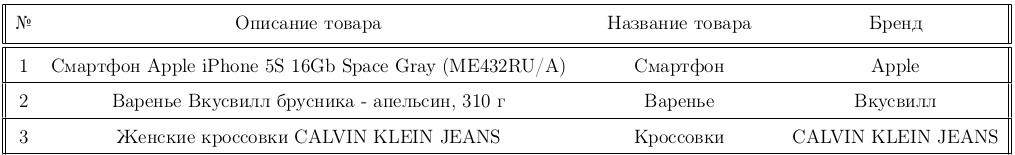
\includegraphics[width=0.7\textwidth]{p1.jpg}
		\label{fig:sample}
	\end{figure}
    
    Тогда поставленную задачу можно решать с помощью распознавания именованных сущностей (NER) в запросах пользователей.
	\begin{figure}[H]
		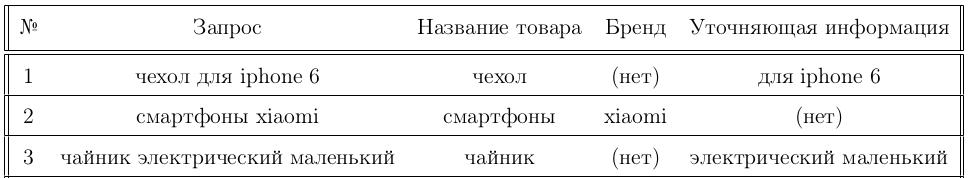
\includegraphics[width=0.7\textwidth]{p2.jpg}
		\label{fig:sample}
	\end{figure}
\end{frame}

\begin{frame}{Особенности сбора данных}
    Названия/описания товаров можно собирать с интернет-магазинов (на практике это нетривиальная задача)\\

	В открытых источниках отсутствуют наборы данных с запросами пользователей, поскольку область сильно коммерциализована.\\
	
	Большое спасибо компании KazanExpress за предоставленный датасет запросов!   
\end{frame}

\begin{frame}{Особенности сбора данных}
    Предложен метод сбора данных-запросов, если нет возможности обратиться к какой-либо компании за данными.
    
    Анализ трафика переходов на сайты интернет-магазинов с поисковиков (Google, Яндекс и т.д.). Существуют сервисы, которые подобные данные предоставляются (ahrefs.com).

	\begin{figure}[H]
		
\includegraphics[width=0.7\textwidth]{ahrefs.jpg}
		\label{fig:sample}
	\end{figure}
\end{frame}

\begin{frame}{Всего собранных данных}
\begin{itemize}
    \item 450.000 товаров, собранных с интернет-магазинов Ozon/Юлмарт/BERU/Яндекс.Маркет
    \item 3.1 млн. товаров, описанных в чеке - с соревнования DataFusion
    \item 3.7 млн. неразмеченных запросов - предоставлены KazanExpress
    \item 10.000 размеченных запросов - немного, т.к. разметка за свой счет
\end{itemize}
\end{frame}

\begin{frame}{Модель}
    BERT для распознавания именованных сущностей. В наиболее похожей по смыслу статье от компании TheHomeDepot использовались рекуррентные модели BiLSTM-CRF и BiGRU. В этом основное отличие моей работы и их статьи.\\\\
    BERT предобучался на всем корпусе текстов на задачу предсказания замаскированных слов, а потом дообучался на задачу NER на небольшом (10.000 сэмплов) размеченном датасете запросов.\\
    

\end{frame}

\begin{frame}{Токенизатор}
    В качестве токенизатора - свой обученный WordPiece. Обучен на всем корпусе текстов (на 30 тыс. токенов). Разбиение на подслова способствует повышению качества модели (т.к. пользователи допускают опечатки в запросах, и, если ошибка произошла, то ошибется только в одном субтокене).
    
	\begin{figure}[H]
		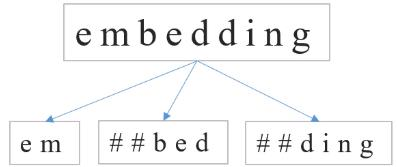
\includegraphics[width=0.5\textwidth]{tok.jpg}
		\label{fig:sample}
	\end{figure}
\end{frame}

\begin{frame}{Лосс на обучении/валидации}
	\begin{figure}[H]
		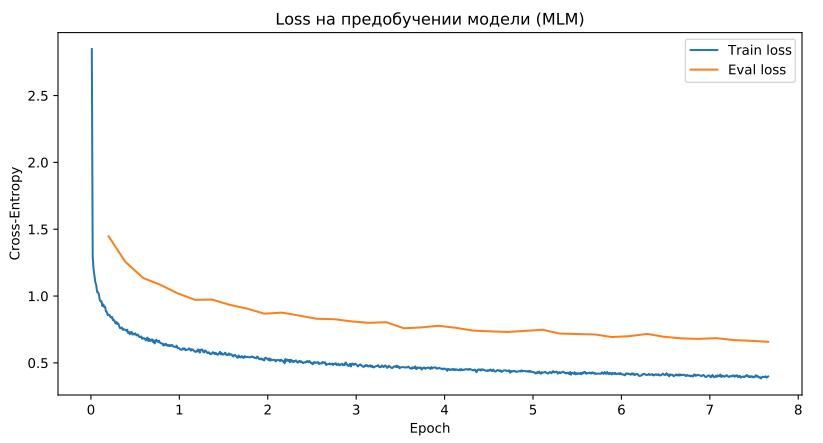
\includegraphics[width=0.45\textwidth]{loss_pretrain.jpg}
		\label{fig:sample}
	\end{figure}

	\begin{figure}[H]
		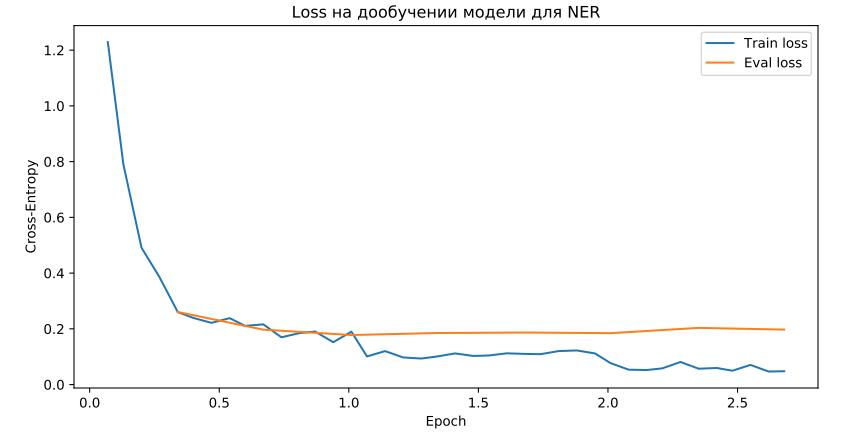
\includegraphics[width=0.45\textwidth]{loss_ner.jpg}
		\label{fig:sample}
	\end{figure}
\end{frame}

\begin{frame}{Пример работы (предсказание маскированных слов)}
	\begin{figure}[H]
		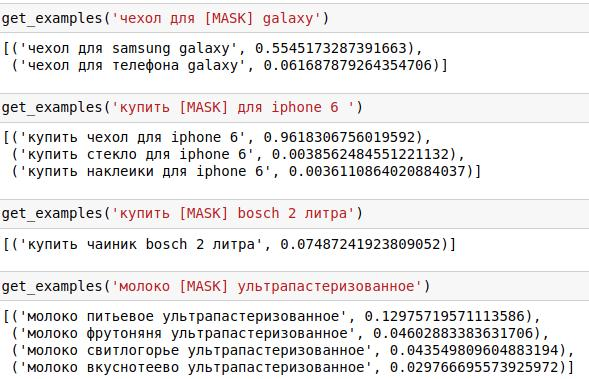
\includegraphics[width=0.45\textwidth]{mlm.jpg}
		\label{fig:sample}
	\end{figure}
	

\end{frame}
\begin{frame}{Пример работы (предсказание маскированных слов)}
	Как бонус - можно использовать для автоматического предложения новых слов запросе
	\begin{figure}[H]
		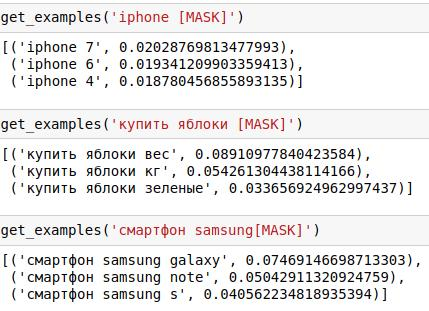
\includegraphics[width=0.45\textwidth]{mlm2.jpg}
		\label{fig:sample}
	\end{figure}
\end{frame}
\begin{frame}{Пример работы (распознавание именованных сущностей)}
	\begin{figure}[H]
		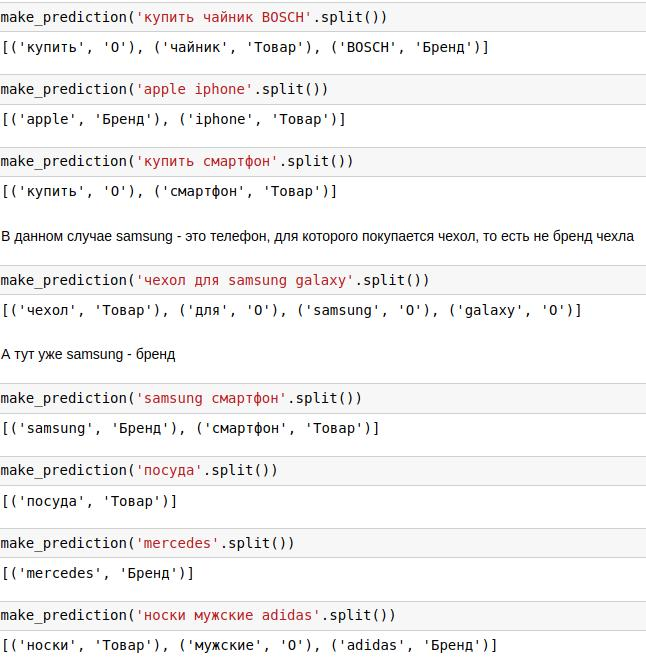
\includegraphics[width=0.45\textwidth]{ner.jpg}
		\label{fig:sample}
	\end{figure}
\end{frame}

\begin{frame}{Приложение}
Весь код и обученные модели доступны на GitHub автора: https://github.com/Sorrow321/cmc\_seminar\\

Можно самостоятельно проверить эксперименты и результаты. Данные для обучения не выкладываются, поскольку была просьба от KazanExpress их не разглашать.
\end{frame}

\begin{frame}{Заключение}
\begin{itemize}
    \item Были указаны ключевые сложности со сбором данных
    \item Был предложен метод сбора запросов пользователей в интернет-магазины через посредников --- общие поисковые системы (Яндекс, Google и т.д.)
    \item Был собран обучающий набор данных, часть из них была вручную размечена
    \item Была предложена нейросетевая архитектура, основанная на BERT, для решения поставленной задачи
    \item Был предложен метод токенизации входных запросов, который способствует более качественной работе модели в случае, когда пользователь допустил опечатку в запросе
    \item Были построены прототипы моделей, решающих поставленные задачи
    \item Был предложен метод предсказания следующего слова в запросе
\end{itemize}
\end{frame}

% Не редактируем: Страница библиографии (формируется автоматически из книжек, указанных в refs.bib и пометок \cite{имя_источника} в тексте)
\include{templates/bib-page}

\end{document}
